\documentclass[pdf]{beamer}
\mode<presentation>{}
\usetheme{Dresden}
\usepackage{apalike}
\usepackage{graphicx}
\usepackage{movie15}
\usepackage{mwe,tikz}
\usepackage[percent]{overpic}
\beamertemplatenavigationsymbolsempty
%% preamble
\title{Non-linear dispersive water wave models}
\usepackage{subcaption}
\author{Jordan Pitt, Stephen Roberts and Christopher Zoppou \\ Australian National University}
\newcommand\solidrule[1][0.25cm]{\rule[0.5ex]{#1}{1pt}}
\newcommand\dashedrule{\mbox{\solidrule[2mm]\hspace{2mm}\solidrule[2mm]}}
\newcommand{\dotrule}[1]{%
	\parbox[]{#1}{\dotfill}}

\setbeamertemplate{itemize item}[triangle]

\newcommand\T{\rule{0pt}{3ex }}       % Top table strut
\newcommand\B{\rule[-4ex]{0pt}{4ex }} % Bottom table strut

\begin{document}

% 'Thriller'	
\begin{frame}[plain]{}
\begin{tikzpicture}[remember picture,overlay]
\node[anchor=north east, inner sep=0pt] at (current page.north east) {
	\includemovie[
	poster,
	text={}
	]{\paperwidth}{\paperheight}{./Videos/Dambreak.avi}
};
\end{tikzpicture}
\end{frame}
	
	
%% title frame
\begin{frame}
\titlepage
\end{frame}
%% normal frame
	

%Do a brief show pictures of water waves, hazards posed
%Move onto the equations, with a picture
%Method: in terms of polynomial representation, FEM, FVM
%Validation: Present results of linear analysis: stability and dispersion analysis, then numerical solution comparisons

\begin{frame}{Outline}
	\begin{itemize}
		\item Motivation
		\item Equations
		\item Linear Theory
		\item Comparison To Numerical Solutions
	\end{itemize}
\end{frame}
\section{Motivation}
%Wave modelling
\begin{frame}{Motivation - Water Waves}
We require accurate models of water waves to understand natural hazards in particular
	\begin{itemize}
		\item Tsunamis
		\item Storm Surges
	\end{itemize}
\end{frame}

\begin{frame}{Motivation}
\begin{figure}
	\centering
	\begin{subfigure}{0.49\textwidth}
		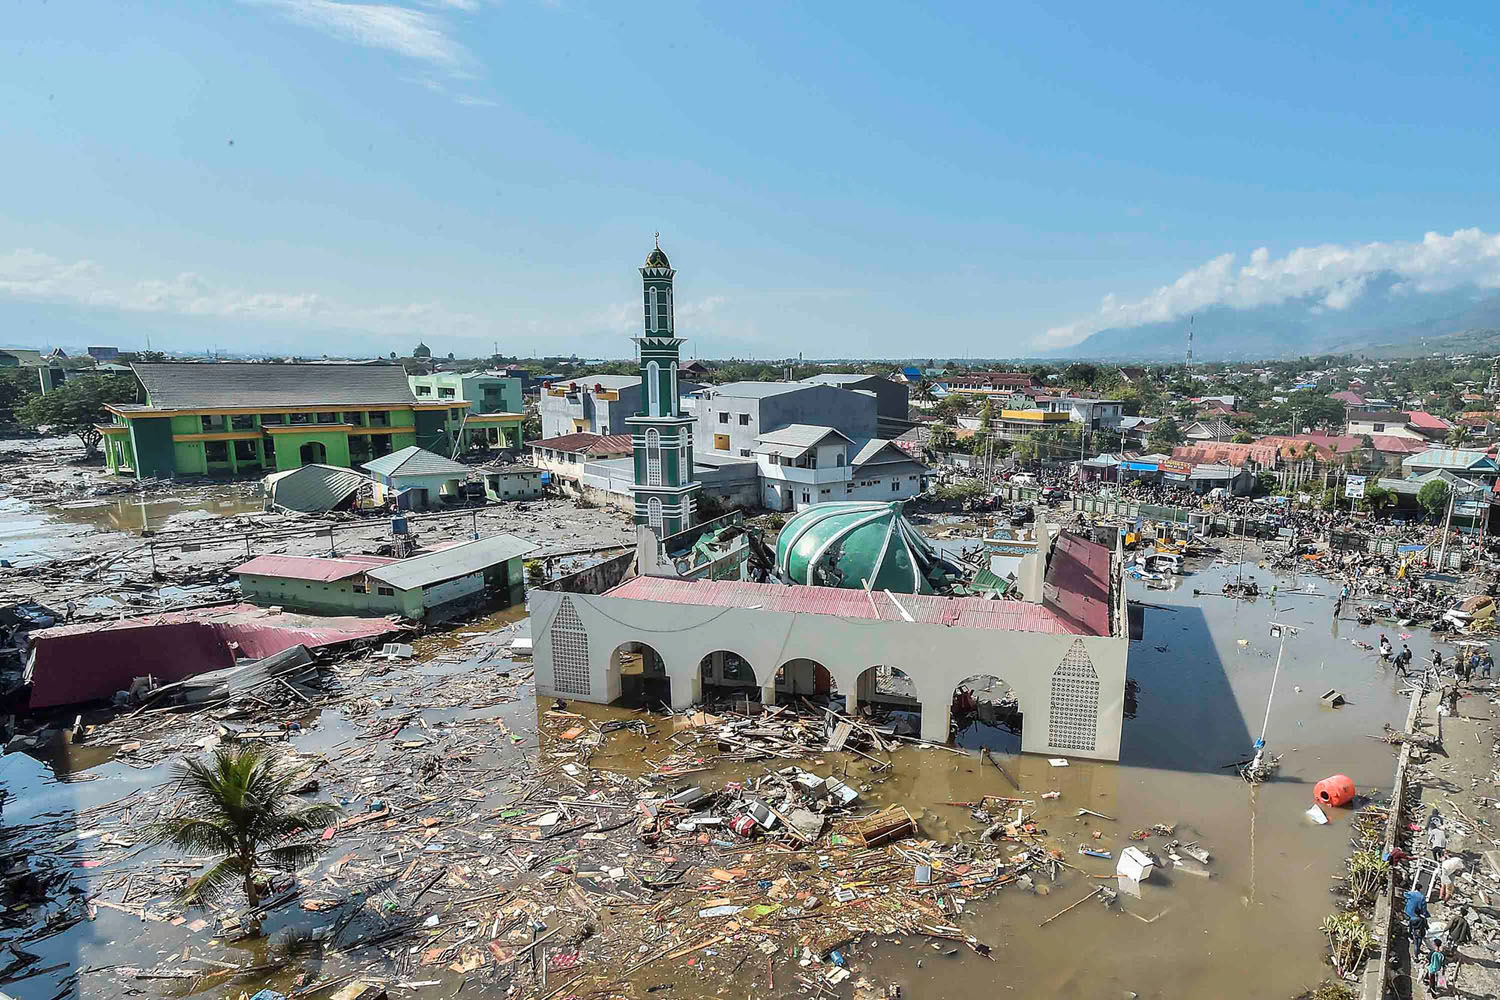
\includegraphics[width=0.9\textwidth]{./Pics/Web/SualwesiTsunami.jpg}
		\caption{Sulawesi Tsunami (Indonesia, 2018).}
	\end{subfigure}
	\begin{subfigure}{0.49\textwidth}
	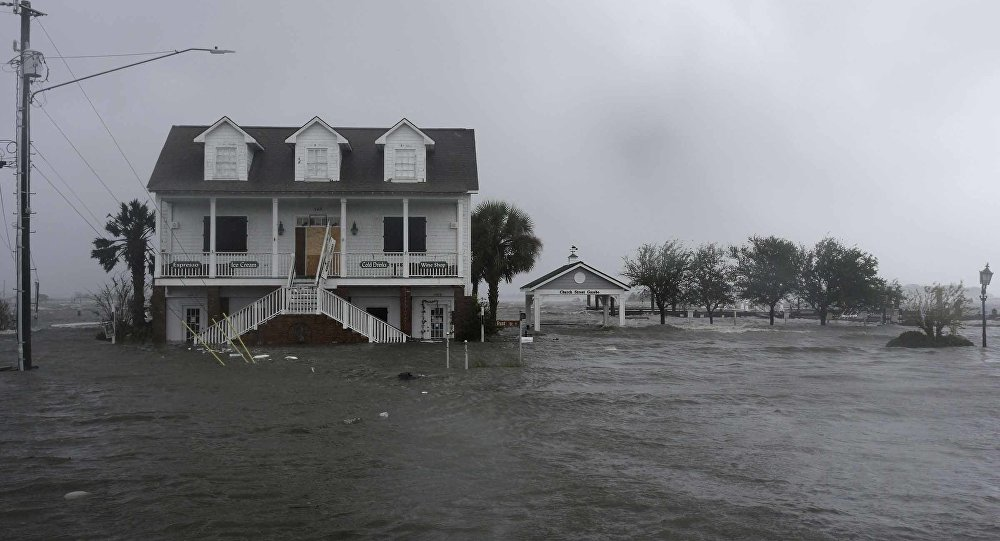
\includegraphics[width=1.1\textwidth]{./Pics/Web/HurricaneFlorence.jpg}
	\subcaption{Hurricane Florence (U.S.A, 2018)}
	\end{subfigure}
\end{figure}
\end{frame}

\begin{frame}{Motivation}
\begin{figure}
	\centering
	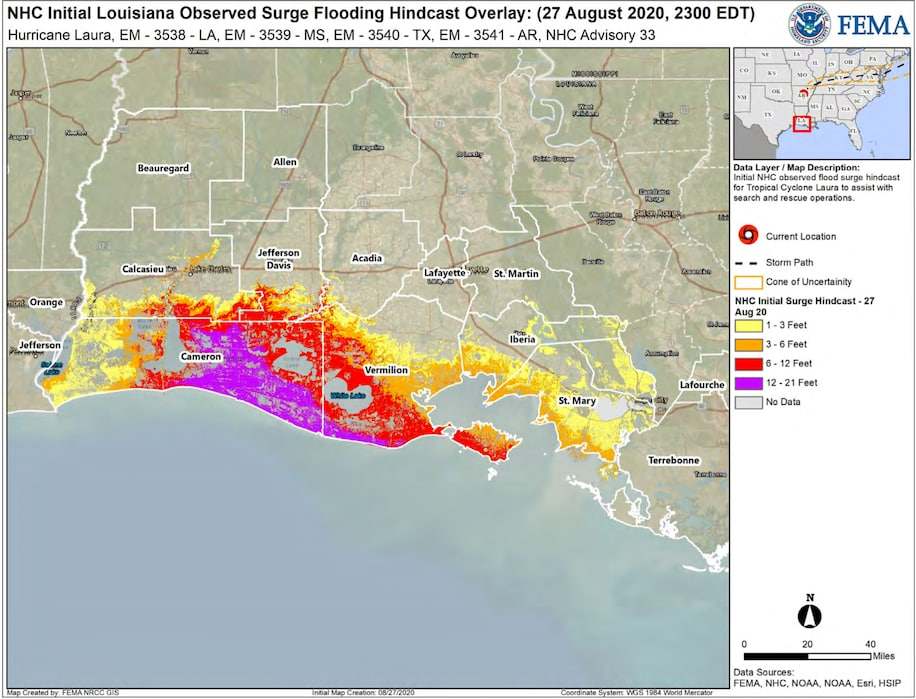
\includegraphics[width=0.7\textwidth]{./Pics/Web/StormSurgeLaura.jpeg}
	\caption{Hurricane Laura (U.S.A, 2020).}
\end{figure}
\end{frame}

\begin{frame}{Motivation - Water Waves}
We require accurate models of water waves to understand natural hazards in particular
\begin{itemize}
	\item Tsunamis
	\item Storm Surges
\end{itemize}
\bigskip
Current models built on non-dispersive models where wave speed independent of frequency (Shallow Water Wave Equations). 
\pause

\bigskip
\textbf{{What's the effect of dispersion on these natural hazards?}}
\end{frame}

\begin{frame}{What's the effect of dispersion on these natural hazards?}
Response:
\begin{itemize}
	\item Compare nonlinear equations/ family of equations with different dispersive properties
	\begin{itemize}
	\item Using their linearised properties - dispersion relationship
	\item Using numerical solutions
	\end{itemize}
\end{itemize}
\bigskip
\pause
\emph{Which family of equations?}
\end{frame}


\section{Family of Equations}
\begin{frame}{Depth Averaged Set Up}
%Equations for conservation of mass and momentum written in terms of the water depth $h(x,t)$, the depth average horizontal velocity $u(x,t)$ and acceleration due to gravity $g$.
\begin{figure}
	\centering
	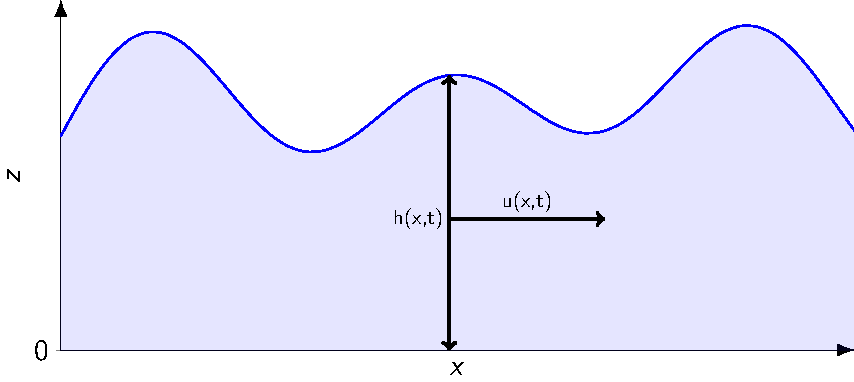
\includegraphics[width=0.9\textwidth]{./Pics/Tex/Explanatory/Setupplot/Waves.pdf}
	\caption{Relevant Quantities.}
\end{figure}
\end{frame}


\begin{frame}{Generalised Serre-Green-Naghdi Equations}
%conservation of mass (exact)
%conservation of momentum (approximation)
%Our h, u and g from before, and also now some free paramters - beta1 and beta2
%Equations also possess an equation for conservation of energy (which holds when quantities are sufficiently smooth)
%when beta's are 0, we get the familar non-dispersive SWWE
%For a physical interpretation, the betas will determine our approximation to the vertical velocity of the water at the free surface, when betas are 0, the vertical velocity is 0, otherwise it is some value dependent on derivatives of h and u in the latter case it is linear throghout depth
\begin{align*}
&\dfrac{\partial h}{\partial t} + \dfrac{\partial (hu)}{\partial x} = 0\\
&\dfrac{\partial (hu)}{\partial t} + \dfrac{\partial }{\partial x} \left( hu^2 + \frac{1}{2}gh^2  +  {\color{blue} {\beta_1} \Phi } -   {\color{red} {\beta_2}\Psi}  \right)= 0 \\
\end{align*}
where
\begin{align*}
\color{blue} \Phi  & \color{blue}= \frac{h^3}{2}\left( \frac{\partial u}{\partial x}\frac{\partial u}{\partial x} - \frac{\partial^2 u}{\partial x \partial t} - u\frac{\partial^2 u}{\partial x^2}\right) \\
\color{red} \Psi & \color{red}=  \frac{gh^2}{2} \left(h \frac{\partial^2 h}{\partial x^2} + \frac{1}{2} \frac{\partial h}{\partial x}\frac{\partial h}{\partial x}\right)
\end{align*}
\end{frame}

\begin{frame}{Generalised Serre-Green-Naghdi Equations - Properties}
\begin{itemize}
	\item Conserves mass, momentum and energy
	\item Reduces to well known equations for particular $\beta$ values
	\item Depth averaged equations have been very successful for large scale models
	\item Nice linear dispersion properties as well
\end{itemize}
\end{frame}

\section{Linear Theory}
\begin{frame}{Linear Dispersion Relationship}
\begin{itemize}
	\item Linearise equations - considering waves of small amplitude (we are going to neglect background velocity ($U$) at first)
	\item Relate angular frequency ($\omega$) to  wave number ($k$)
\end{itemize}
\end{frame}

    
    
%Considering wave properties of small amplitude waves on a large background of still water
\begin{frame}{Linearise equations (Space)}
\begin{figure}
	\centering
	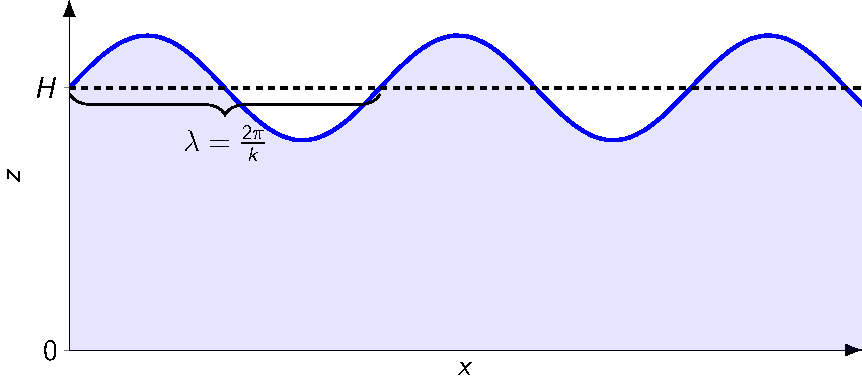
\includegraphics[width=0.9\textwidth]{./Pics/Tex/Explanatory/DispersionPlot/Dispersion.pdf}
\end{figure}
\end{frame}

\begin{frame}{Linearise equations (Space/ {\color{red} Time})}
\begin{figure}
	\centering
	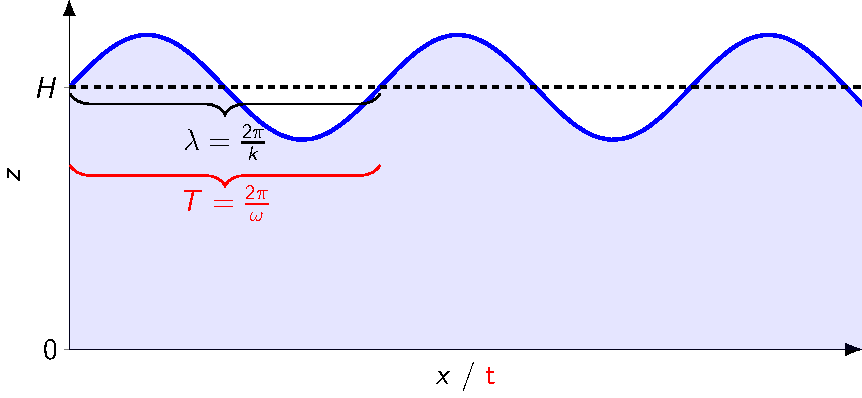
\includegraphics[width=0.9\textwidth]{./Pics/Tex/Explanatory/DispersionPlot/Dispersion_Analagous.pdf}
\end{figure}
\end{frame}

\begin{frame}{Dispersion Relations of generalised Serre-Green-Naghdi and Water (linearised)}
\begin{align*}
\omega_{\text{gSGN}}^2 & = gH k^2 \dfrac{{\color{red}\beta_2 H^2 k^2} + 2}{ {\color{blue}\beta_1 H^2 k^2} + 2} \\
\omega_{\text{water}}^2 & = gk \tanh\left(kH\right)
\end{align*}
\end{frame}

\begin{frame}{Taylor Series Expansions}
\begin{align*}
\omega_{\text{gSGN}}^2 & = gH k^2 &&-\frac{ {\color{blue}\beta_1} - {\color{red}\beta_2}  }{2} g H^3  k^4 &&+ \frac{{\color{blue}\beta_1}\left({\color{blue}\beta_1}- {\color{red}\beta_2}\right) }{4}  g H^5 k^6 &&+ \mathcal{O}\left(k^8\right)\\
\omega_{\text{water}}^2 & = gH k^2 &&-\frac{1}{3}gH^3 k^4   &&+ \frac{2}{15} gH^5 k^6  &&+ \mathcal{O}\left(k^8\right) 
\end{align*}
\pause
So 
\begin{table}
\begin{tabular}{c | c}
${\color{blue}\beta_1} - {\color{red}\beta_2}  = 0$ & $\mathcal{O}\left(k^2\right) $ Accurate (Non-dispersive)\\
${\color{blue}\beta_1} - {\color{red}\beta_2}  = 2/3$ & $\mathcal{O}\left(k^4\right) $ Accurate \\
${\color{blue}\beta_1} - {\color{red}\beta_2}  = 2/3$ and ${\color{blue}\beta_1} = \frac{4}{5}$  & $\mathcal{O}\left(k^6\right) $ Accurate \\
\end{tabular}
\end{table}
\end{frame}


\begin{frame}{Accuracy Summary Plot}
\centering
	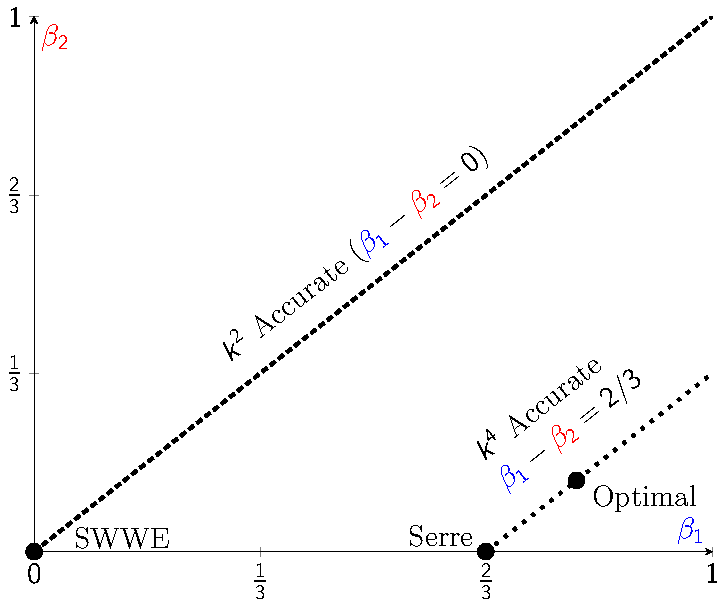
\includegraphics[width=0.75\textwidth]{./Pics/Tex/Explanatory/RegionsPlot/AccuracySummary.pdf}
\end{frame}

\begin{frame}{Phase Speed ($c$)}

$$c_{\text{gSGN}}^2 = \dfrac{\omega_{\text{gSGN}}^2}{k^2} = gH \dfrac{{\color{red}\beta_2 H^2 k^2} + 2}{ {\color{blue}\beta_1 H^2 k^2} + 2} $$
\\
\pause
We will now allow non-zero background velocities ($U$) and no longer look at the square of the phase speed (resulting in negative and positive branches). Thus we get
\begin{align*}
c^+_{\text{gSGN}} &= U + \sqrt{gH} \sqrt{ \dfrac{{\color{red}\beta_2 H^2 k^2} + 2}{ {\color{blue}\beta_1 H^2 k^2} + 2}} \\
c^-_{\text{gSGN}} &= U - \sqrt{gH} \sqrt{ \dfrac{{\color{red}\beta_2 H^2 k^2} + 2}{ {\color{blue}\beta_1 H^2 k^2} + 2}}
\end{align*}

\end{frame}

\begin{frame}{Phase Speed ($c$)}
The important term here in terms of dispersive properties and the effect of $\beta$ values is
\[\sqrt{ \dfrac{{\color{red}\beta_2 H^2 k^2} + 2}{ {\color{blue}\beta_1 H^2 k^2} + 2}}\]
In particular we have that 
\begin{itemize}
	\item this term is monotone for $k \ge 0 $
	\item $\sqrt{ \frac{{\color{red}\beta_2 H^2 k^2} + 2}{ {\color{blue}\beta_1 H^2 k^2} + 2}} \rightarrow 1 $ as $k \rightarrow 0$
	\item $\sqrt{ \frac{{\color{red}\beta_2 H^2 k^2} + 2}{ {\color{blue}\beta_1 H^2 k^2} + 2}} \rightarrow \sqrt{\frac{{\color{red}\beta_2 }}{{\color{blue}\beta_1 }}} $ as $k \rightarrow \infty$
		\item  $ \sqrt{\frac{{\color{red}\beta_2 }}{{\color{blue}\beta_1 }}} \le
	\sqrt{ \frac{{\color{red}\beta_2 H^2 k^2} + 2}{ {\color{blue}\beta_1 H^2 k^2} + 2}} \le  1$  when ${\color{blue}\beta_1 } > {\color{red}\beta_2 }$
	\item $1 \le \sqrt{ \frac{{\color{red}\beta_2 H^2 k^2} + 2}{ {\color{blue}\beta_1 H^2 k^2} + 2}} \le  \sqrt{\frac{{\color{red}\beta_2 }}{{\color{blue}\beta_1 }}}$ when ${\color{blue}\beta_1 } < {\color{red}\beta_2 }$ 
\end{itemize}

\end{frame}


\begin{frame}{Phase Speed Regions }
These properties result in the following cases and associated chain of inequalities
\begin{itemize}
\item When ${\color{blue}\beta_1 } > {\color{red}\beta_2 }$ we have
{\footnotesize  \[U - \sqrt{gH}\le   c^-_{\text{gSGN}} \le  U - \sqrt{\frac{{\color{red}\beta_2 }}{{\color{blue}\beta_1 }}} \sqrt{gH} \le 0 \le  U + \sqrt{\frac{{\color{red}\beta_2 }}{{\color{blue}\beta_1 }}} \sqrt{gH} \le c^+_{\text{gSGN}} \le U + \sqrt{gH} \]}
\item When ${\color{blue}\beta_1 } = {\color{red}\beta_2 }$ we have
\[U - \sqrt{gH} =   c^-_{\text{gSGN}} \quad \quad \text{and} \quad \quad  U + \sqrt{gH} =   c^+_{\text{gSGN}}\]
\item When ${\color{blue}\beta_1 } < {\color{red}\beta_2 }$ we have
{\footnotesize \[U - \sqrt{\frac{{\color{red}\beta_2 }}{{\color{blue}\beta_1 }}} \sqrt{gH}\le   c^-_{\text{gSGN}} \le  U - \sqrt{gH} \le 0 \le  U + \sqrt{gH} \le c^+_{\text{gSGN}} \le U +  \sqrt{\frac{{\color{red}\beta_2 }}{{\color{blue}\beta_1 }}} \sqrt{gH}  \]}
\end{itemize}
\end{frame}


\begin{frame}{Phase Speed Regions }
Since $U - \sqrt{gH} $  and $U +  \sqrt{gH} $ will bound location of the shocks we have that
\begin{itemize}
	\item When ${\color{blue}\beta_1 } > {\color{red}\beta_2 }$ we have dispersive waves form behind shocks
	\item When ${\color{blue}\beta_1 } = {\color{red}\beta_2 }$ we have no dispersive waves
	\item When ${\color{blue}\beta_1 } < {\color{red}\beta_2 }$ we have dispersive waves form ahead of shocks 
\end{itemize}
\end{frame}
\begin{frame}{Accuracy Summary Plot}
\centering
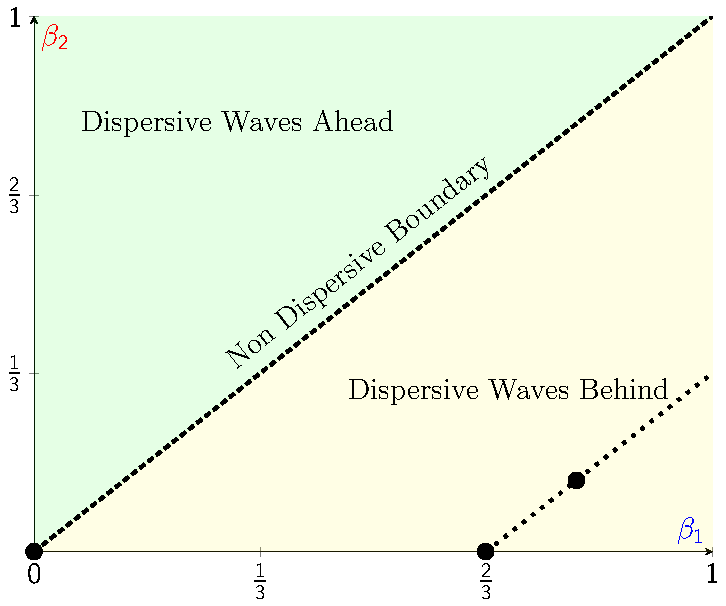
\includegraphics[width=0.75\textwidth]{./Pics/Tex/Explanatory/RegionsPlot/AccuracySummaryWithRegions.pdf}
\end{frame}

\section{Comparison To Numerical Solutions}
\begin{frame}{Comparsion Between Linear Theory and Numerical Solutions}
Look at a solutions of the Dam break problem initial condition for
\begin{itemize}
	\item Fixed $\beta$ values
	\item Changing $\beta$ values
\end{itemize}
\end{frame}

\begin{frame}{Dambreak Problem Initial Conditions}
\centering
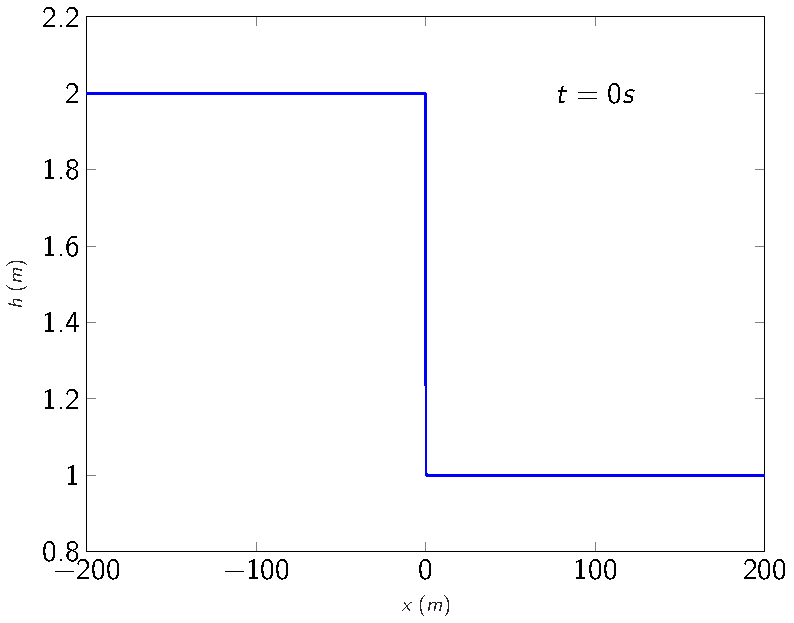
\includegraphics[width=0.73\textwidth]{./Pics/Tex/Results/DB/Init/Init.pdf}
\end{frame}

\begin{frame}{Shallow Water Wave Equations \hfill 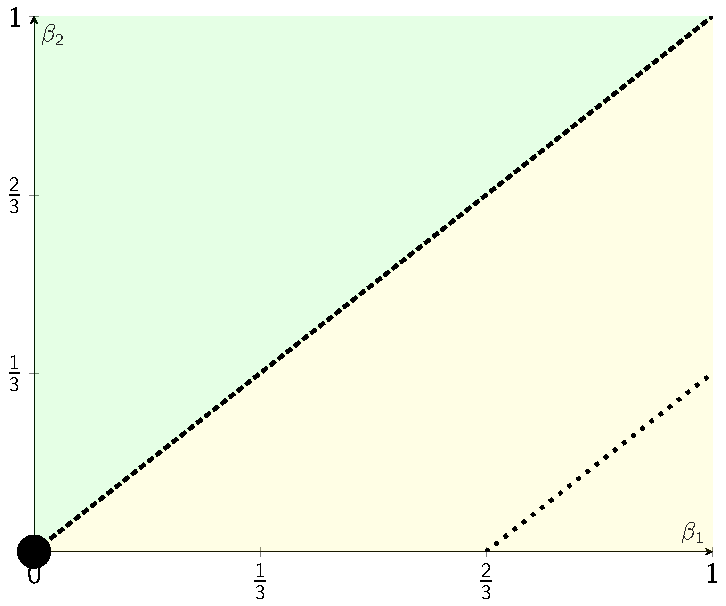
\includegraphics[width=0.17\textwidth]{./Pics/Tex/Explanatory/RegionsPlot/SPSWWE.pdf}}
\centering
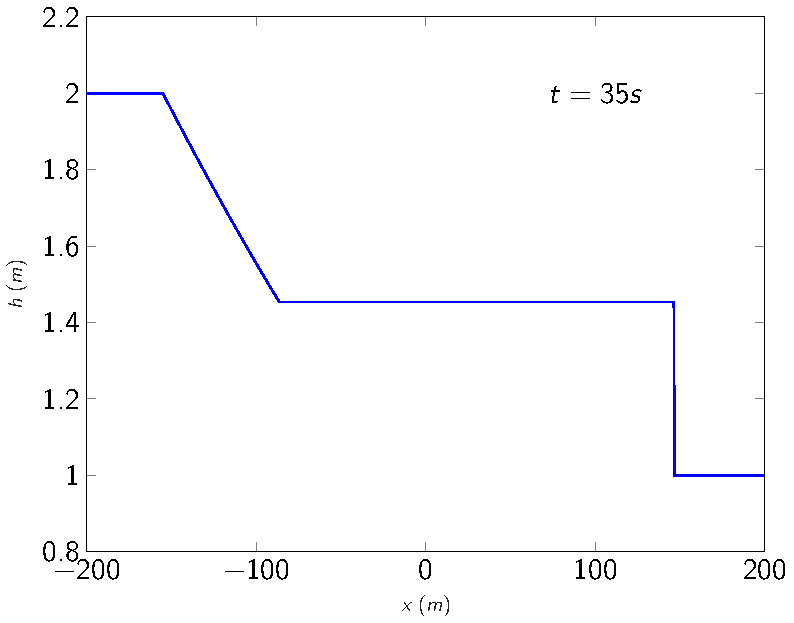
\includegraphics[width=0.7\textwidth]{./Pics/Tex/Results/DB/SWWE/SWWE.pdf}
\end{frame}

\begin{frame}{Shallow Water Wave Equations \hfill 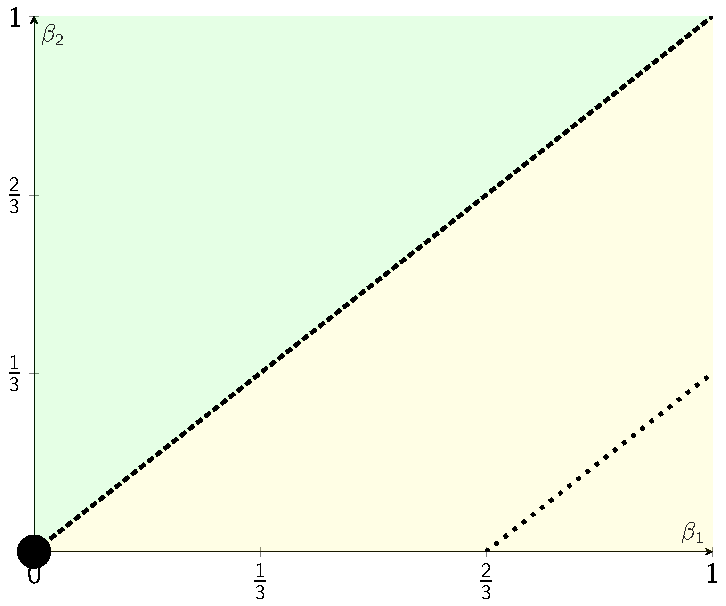
\includegraphics[width=0.17\textwidth]{./Pics/Tex/Explanatory/RegionsPlot/SPSWWE.pdf}}
\centering
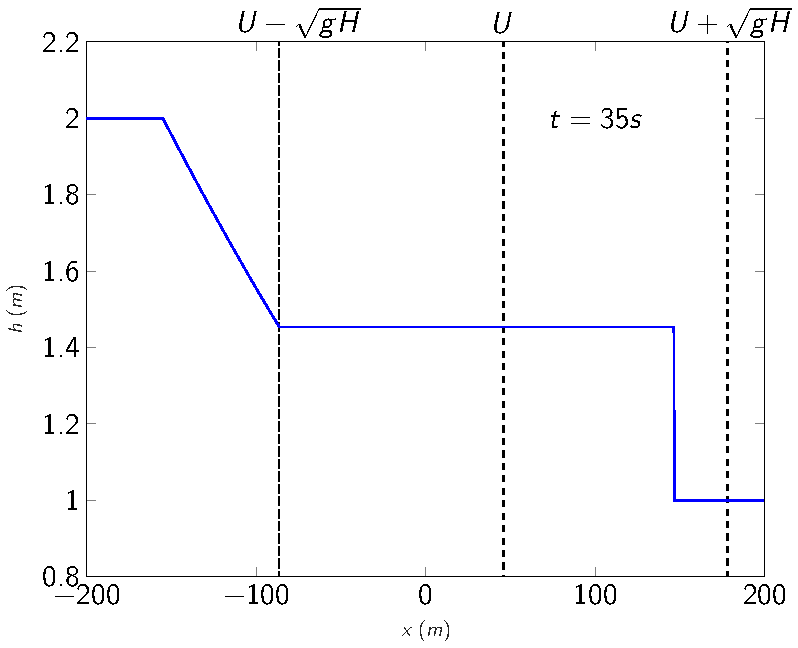
\includegraphics[width=0.7\textwidth]{./Pics/Tex/Results/DB/SWWE/RegionSWWE.pdf}
\end{frame}


\begin{frame}{Other Non-Dispersive Equations \hfill 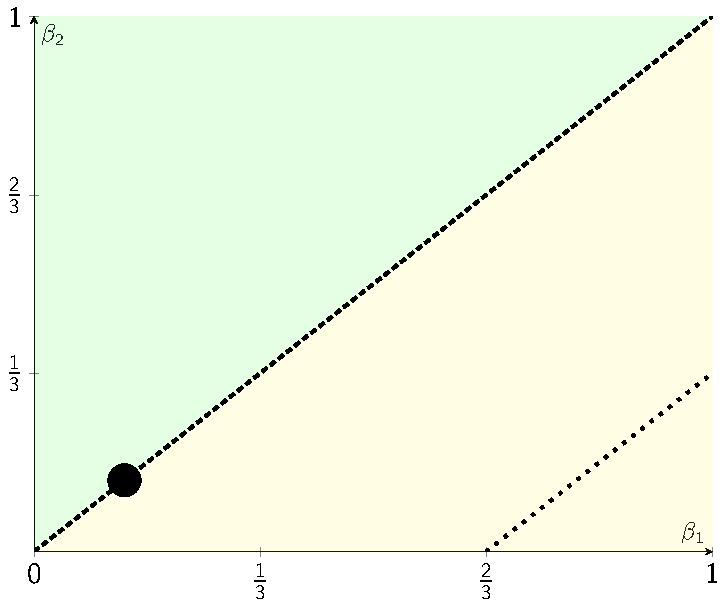
\includegraphics[width=0.17\textwidth]{./Pics/Tex/Explanatory/RegionsPlot/SPrSV.pdf}}
\centering
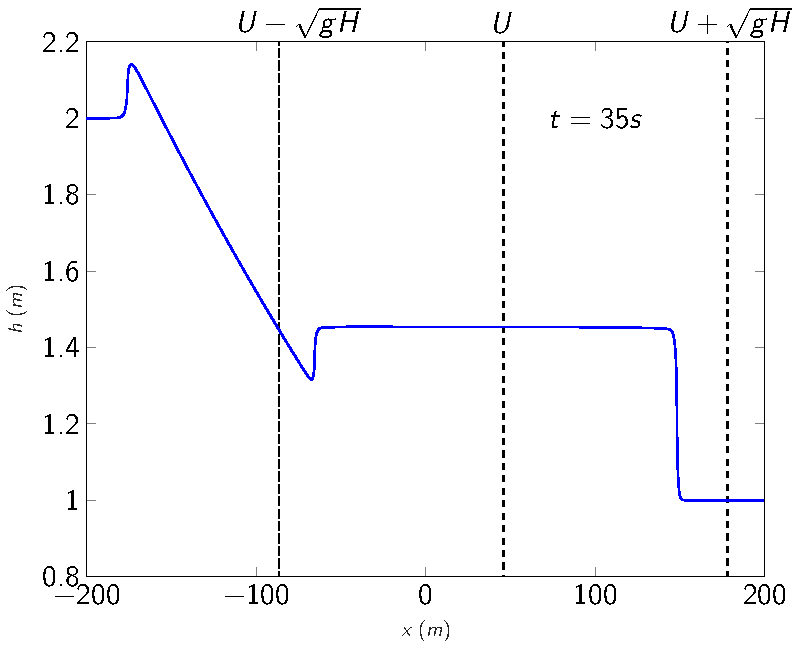
\includegraphics[width=0.7\textwidth]{./Pics/Tex/Results/DB/rSV/RegionrSV.pdf}
\end{frame}

\begin{frame}{Serre Equations \hfill 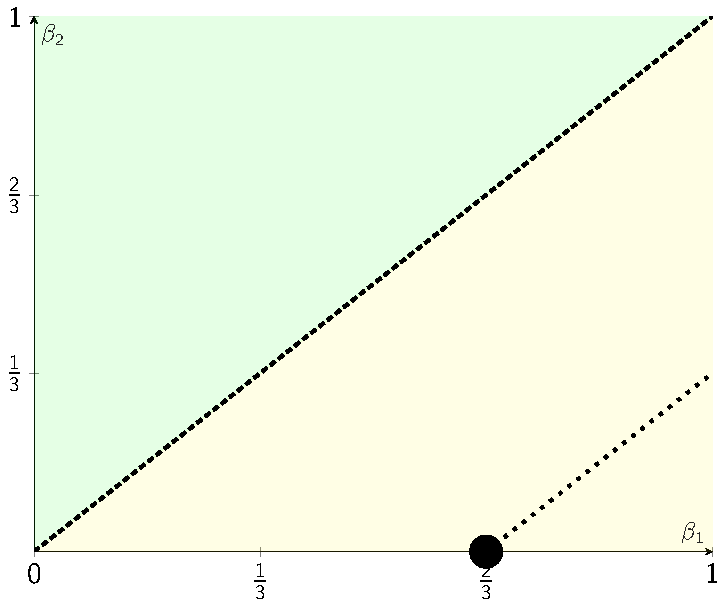
\includegraphics[width=0.17\textwidth]{./Pics/Tex/Explanatory/RegionsPlot/SPSerre.pdf}}
\centering
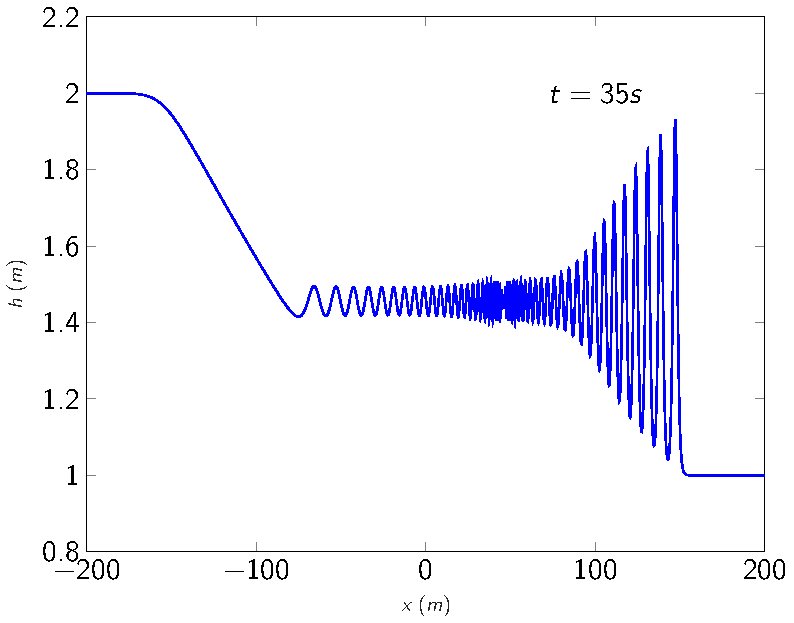
\includegraphics[width=0.7\textwidth]{./Pics/Tex/Results/DB/Serre/Serre.pdf}
\end{frame}

\begin{frame}{Serre Equations \hfill 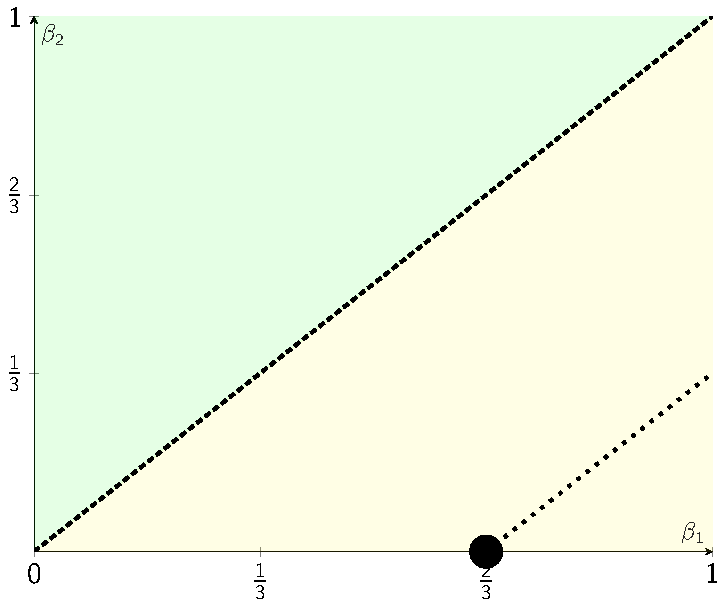
\includegraphics[width=0.17\textwidth]{./Pics/Tex/Explanatory/RegionsPlot/SPSerre.pdf}}
\centering
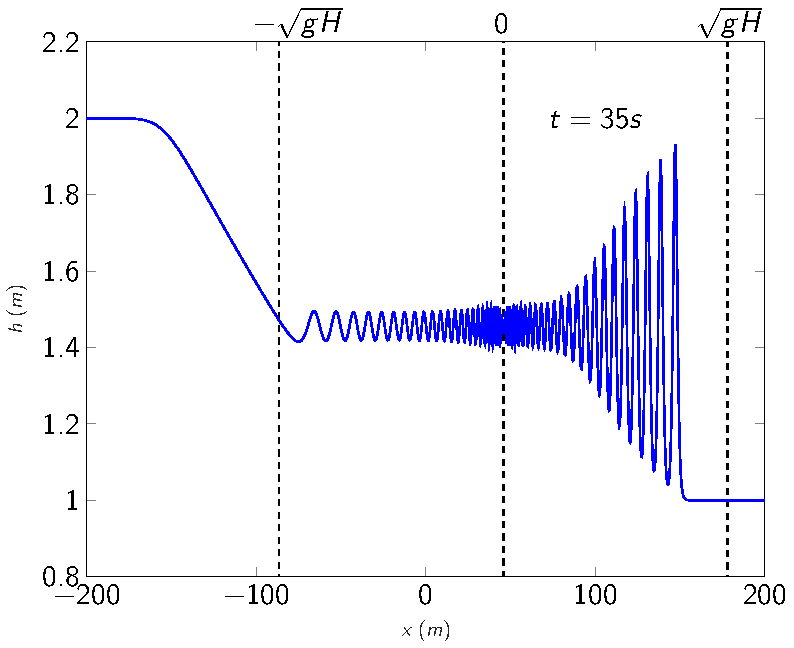
\includegraphics[width=0.7\textwidth]{./Pics/Tex/Results/DB/Serre/RegionSerre.pdf}
\end{frame}

\begin{frame}{Optimal Dispersion Equations \hfill 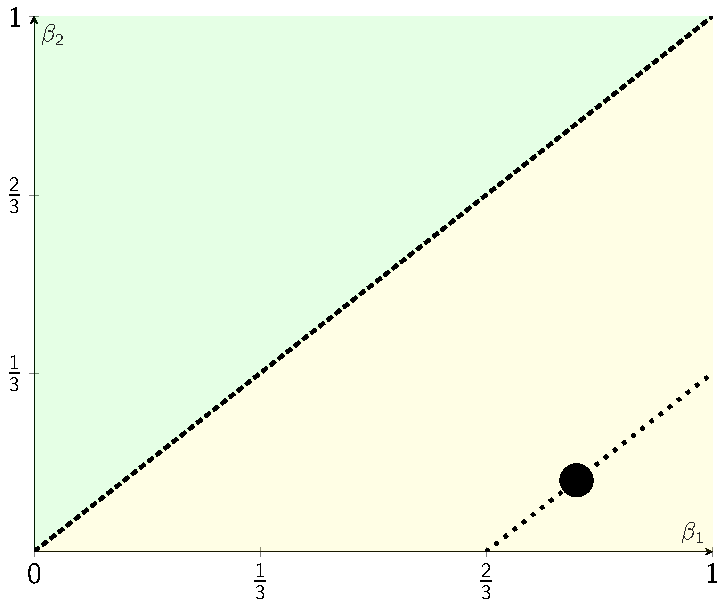
\includegraphics[width=0.17\textwidth]{./Pics/Tex/Explanatory/RegionsPlot/SPiSGN.pdf}}
\centering
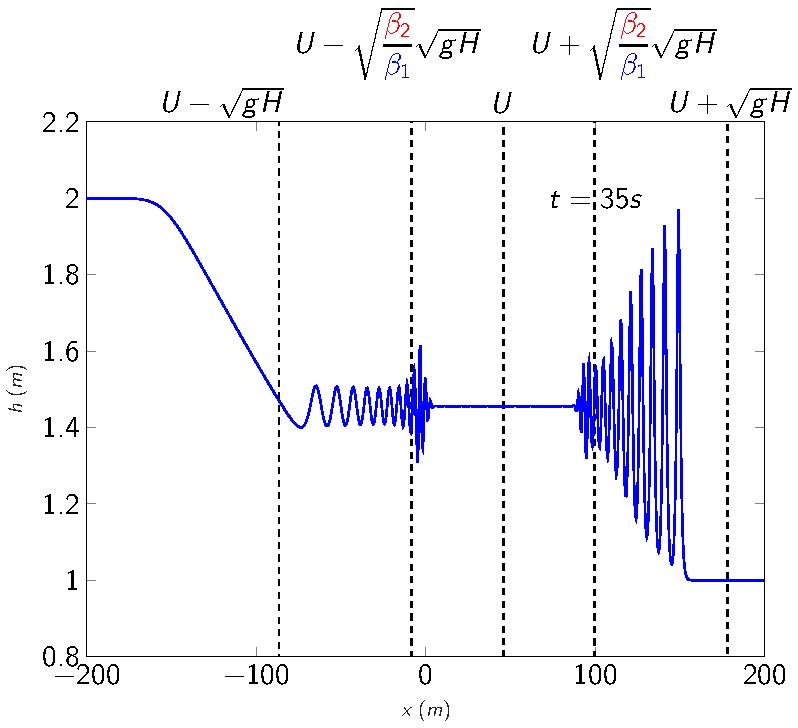
\includegraphics[width=0.62\textwidth]{./Pics/Tex/Results/DB/iSGN/RegioniSGN.pdf}
\end{frame}

\begin{frame}{Changing $\beta$ values}
Now that we have gone through in depth each of the particular $\beta$ values, we can begin to understand what happens if we change $\beta$ values over time. Coming back to the original video at the beginning of the talk.
\end{frame}

\begin{frame}{Changing $\beta$ values Outline}
\centering
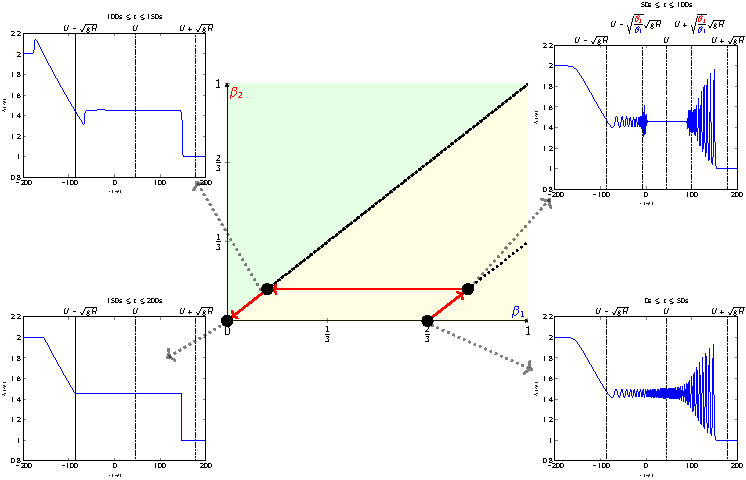
\includegraphics[width=0.99\textwidth]{./Pics/Tex/Explanatory/RegDBV/3x3Grid.pdf}
\end{frame}

\begin{frame}[plain]{}
\begin{tikzpicture}[remember picture,overlay]
\node[anchor=north east, inner sep=0pt] at (current page.north east) {
	\includemovie[
	poster,
	text={}
	]{\paperwidth}{\paperheight}{./Videos/Dambreak.avi}
};
\end{tikzpicture}
\end{frame}

\begin{frame}
Thanks\end{frame}

\end{document}